\documentclass{report}
\usepackage{listings}
\usepackage{graphicx}
\usepackage[usenames]{color}
\usepackage[english]{babel}

\definecolor{darkblue}{rgb}{0,0.08,0.45}
\definecolor{lightgrey}{rgb}{0.97,0.97,0.97}
\definecolor{lightgreen}{rgb}{0.13,0.54,0.13}
\definecolor{lightblue}{rgb}{0.33,0.33,0.74}
\definecolor{lightred}{rgb}{0.54,0.13,0.13}

\lstset{frame=lines, numbers=left, frameround=ffff,
commentstyle=\color{lightblue}, stringstyle=\color{lightred},
keywordstyle=\color{lightgreen}, backgroundcolor=\color{lightgrey},
showstringspaces=false}

\begin{document}

%
% TITLE
%
\title
{
    \textcolor{darkblue}{Multitouch library} 1.0.0 \\
    \textbf{Driver Development Guideline}
}
\author
{
    David Keller \\ 
    \textless\textcolor{darkblue}{\texttt{keller@efrei.fr}}\textgreater
}
\date{\today}
\maketitle

%
% ABSTRACT
%
\begin{abstract}
This document is intended for developers who want to use the 
\textcolor{darkblue}{Multitouch} library to fit particular purposes.
It describes the part of the library api dedicated to the extensions,
and shows some examples.
\end{abstract}

%
% TABLE OF CONTENTS
%
\tableofcontents
\pagestyle{headings}

%
% CONTENTS
%
\part{\textcolor{darkblue}{Introduction}}
The \textcolor{darkblue}{Multitouch} library is able to suit different setups 
\& needs by loading modules which change its behavior.

The library architecture remains simple and provides two main entities:
\begin{itemize}
\item \textit{inputs} that generate packets.
\item \textit{outputs} that are responsible of final processing on packets. 
\end{itemize}
An application can enable as many inputs \& outputs as needed, may use
them independently or bind inputs to outputs (this is the standard
behavior as shown in the image).
\begin{center}
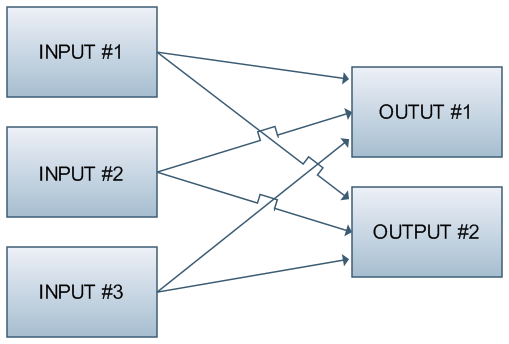
\includegraphics[keepaspectratio=true, width=200pt]{images/arch.png}
\end{center}

Also as you can see in the following image, inputs transmit 
packets to processing engines before making them available to the application
(or straight to outputs), and outputs pass the packets they receive from the 
application (or directly from inputs) to processing engines too, before doing 
own processing on them.
\begin{center}
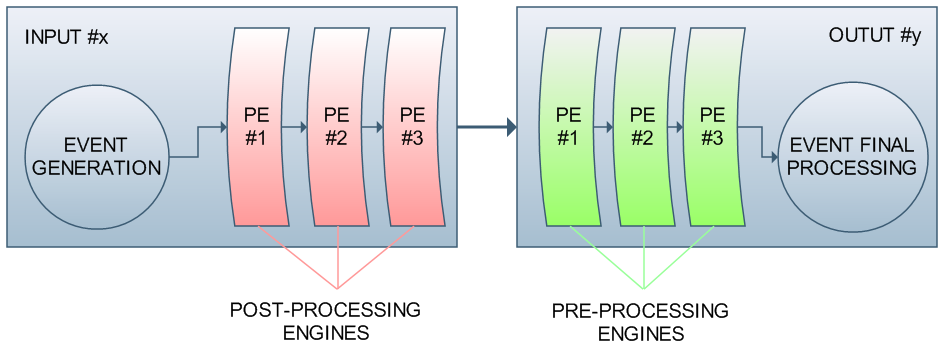
\includegraphics[keepaspectratio=true, width=\textwidth]{images/arch_pe.png}
\end{center}

To customize the inputs, outputs and processing engines to fit your
requirements and hardware, you have to write drivers (a driver is 
composed of three \texttt{C} functions which respect a defined prototype).

Thanks to this modular design and drivers, you could use the 
\textcolor{darkblue}{Multitouch} library to offer to an application 
the possibility to:
\begin{itemize}
\item Get datas from a touchpad or from more than one device (using or 
\textbf{not}, the same driver).
\item Write datas into a file.
\item Merge them and send it over the network
\item Emulate a kernel driver by creating a device on the file system feeded 
by data collected over the network
\item ect..
\end{itemize}

This guide cover all the aspects of the customization of the libary by a
developer, thus it:
\begin{enumerate}
\item Explains how to write a module.
\item Describes inputs drivers. 
\item Describes outputs drivers. 
\item Describes processing engine hook points. 
\end{enumerate}


\part{\textcolor{darkblue}{Modules}}
\chapter{Modules}
The \textcolor{darkblue}{Multitouch} library provide a way to inject code into 
an application during runtime: modules. They are mainly used to add inputs,
outputs and processing engine drivers, but could serve other purposes.
In addition, \textcolor{darkblue}{Multitouch}'s library checks module 
dependencies.

Modules must contains at least two functions, \texttt{init} 
(see \ref{sect:module_init}) \& \texttt{exit} (\ref{sect:module_exit}), 
which are used to handle the module, registered using a \texttt{C} 
pre-processing macro (\ref{sect:module_registration}).
When a module is loaded, the library ensures that its dependencies are 
respected (abort with an error message if \textbf{not}), then it calls the 
\textit{module's init function}. When the application does \textbf{not} need 
it anymore, the \textit{module's exit function} is called, and the module 
is detached.

Section \ref{sect:module_example} shows an example of a complete module.

%
% SECTION Init
%
\section{init}
\label{sect:module_init}
The \textit{init function} of your module is called when it is loaded. This 
function should register your module's content with an application.
It does \textbf{not} take argument but returns an error code, which equals 
\texttt{0} if the function succeed, else the application will be notified by 
the \textcolor{darkblue}{Multitouch} library that an error occured:
% module init Figure
\begin{lstlisting}[language=C, caption=Module's init function example]
/* static means the function is not exported directly to
 * the application, to prevent conflict 
 */
static int
example_module_init(void)
{
    /* Print a message in the console */
    peach_log_info("Example module loaded!\n");

    /* Exit with success */
    return 0; 
}
\end{lstlisting}

This function is \textbf{not} a \textit{drivers's init function} as 
described later in this document. For example, if your module declares two
different drivers, with their respective \textit{drivers's init function}.
Your source file should contain \textbf{two} \textit{drivers's init function} 
and \textbf{one} \textit{module's init function} (that you use to register your
two drivers).




%
% SECTION Exit
%
\section{exit}
\label{sect:module_exit}
The \textit{exit function} is called when the module is unloaded. Like the 
\textit{init function}, it does \textbf{not} take argument but returns an 
error code:
% module exit Figure
\begin{lstlisting}[language=C, caption=Module's exit function example]
static int
example_module_exit(void)
{
    peach_log_info("Example module unloaded!\n");

    return 0; 
}
\end{lstlisting}

This function is a good place to unregister the content of your module to
prevent the application from using it whereas it is \textbf{not} available 
anymore.

%
% SECTION Registration
%
\section{Registration}
\label{sect:module_registration}
A module needs some informations to be loadable:
\begin{itemize}
\item a \textit{name}.
\item a \textit{version number}.
\item its \textit{init function}'s address.
\item its \textit{exit function}'s address.
\item its \textit{depencies} with other modules.
\end{itemize}
Theses informations are saved by two \texttt{C} pre-processing macros:
\begin{itemize}
\item \texttt{PEACH\_MODULE\_REGISTER}.
\item \texttt{PEACH\_MODULE\_DEPENDENCIES}.
\end{itemize}
The name and the version will be used by the \textcolor{darkblue}{Multitouch}
library's dependencies resolver. The name and version of a dependencie must
match exactly the name and the version of a loaded module. The library does 
\textbf{not} assert that a loaded module, with a greater version, is compatible
with a request of a lower version module.

%
% SUBSECTION L_MODULE_REGISTER
%
\subsection{PEACH\_MODULE\_REGISTER}
This macros's arguments are:
\begin{enumerate}
\item the \textit{module name}, a \texttt{C} string.
\item the \textit{module version}, a \texttt{C} \texttt{uint\_64\_t}.
\item the \textit{module init function}, a function pointer (i.e function name).
\item the \textit{module exit function}, a function pointer (i.e function name).
\end{enumerate}

%
% SUBSECTION L_MODULE_DEPENDENCIES
%
\subsection{PEACH\_MODULE\_DEPENDENCIES}
This pre-processing macro takes a list of \texttt{PEACH\_MODULE\_NEED} macros 
as arguments. The macro \texttt{PEACH\_MODULE\_NEED} takes two arguments:
\begin{enumerate}
\item the \textit{requested module name}, a \texttt{C} string.
\item the \textit{requested module version}, a \texttt{C} \texttt{uint\_64\_t}.
\end{enumerate}
If it is \textbf{not} passed argument or if not presented, the library asserts
that the module does \textbf{not} have any dependencie!


%
% SECTION COMPILATION
%
\section{Compilation}
Your module must compiled with the same flags used to compile 
\textcolor{darkblue}{Multitouch} library (e.g. optimization, debug), and be 
linked with it. If you have the \textcolor{darkblue}{Multitouch} project's 
source tree, you just have to reference your module's source file in the 
\texttt{CMakeList.txt} file located in the root directory as shown in the 
following figure:
% configuration Figure
\begin{lstlisting}[language=make, caption=CMakeList.txt update]
# This block schedules the compilation of 
# module/my_module.c (your source file) to create 
# 'my_module'  object.
add_library(
    my_module
    MODULE

    module/my_module.c
)

# This block tells that our object should be linked 
# with the 'multitouch' library.
target_link_libraries(
    my_module

    multitouch
)

# And this block controls the name of the generated
# module.
set_target_properties(
    my_module
    PROPERTIES

    PREFIX ""
    SUFFIX ${MODULE_EXTENSION}
)
\end{lstlisting}

%
% SECTION Complete module example
%
\section{Complete module example}
\label{sect:module_example}
Here is a complete module example which does \texttt{not} contain
any driver:
\begin{lstlisting}[language=C, caption=Complete module example]
/* You can choose any name you desire for this function
 * as long as it is corresponding to the name passed in 
 * the PEACH_MODULE_REGISTER macro 
 */
static int
example_module_init(void)
{
    /* Here is where you may call the functions to 
     * register the drivers you have written into this 
     * source file 
     */
    return 0; 
}

static int
example_module_exit(void)
{
    /* And here is where you unregister them */
    return 0; 
}

/* Your module is named "example_module" version 00 of 
 * the 11 of January 2009 
 */
PEACH_MODULE_REGISTER("example_module", 2009011100,
    example_module_init,
    example_module_exit)

/* It needs two modules: "needed_module" version 
 * 2008122701 and "other_needed_module" version 
 * 2008121100 
 */
PEACH_MODULE_DEPENDENCIES(
    PEACH_MODULE_NEED("needed_module", 2008122701),
    PEACH_MODULE_NEED("other_needed_module", 2008121100))

\end{lstlisting}



\part{\textcolor{darkblue}{Drivers}}
\chapter{Processing engines}

Processing engines are designed to extra process packets. Processing
engines can be chained to permit multiple extra processings. You can
view them as protocols of a one-way network stack. When a packet
enters in this one-way stack, it pass through the first processing engine 
of the stack, and if this processing engine accepts the packet, it is 
processted to the next processing engine, and so on until it reachs the
last processing engine. In the end, the packet can be read on the top of 
the stack.
Processing engines are implemented using the 
\textcolor{darkblue}{Multitouch}'s \texttt{mt\_chain\_} api. This api
offers to the developper the possibility to inject custom processing engine 
logic, by writting a processing engine's driver.

%
% SECTION Where are they used
%
\section{Where are they used ?}

Each \texttt{inputs} \& \texttt{outputs} use processing engines to 
respectively perform post-processing on emited packets and 
pre-processing on received packets. 

%
% SECTION How to write a processing engine
%
\section{How to write a processing engine driver}

A processing engine (i.e. \texttt{mt\_chain\_layer\_t}) use a set of three 
functions written by the module developer: \texttt{init} 
(described section \ref{sect:pengine_init}), \texttt{destroy} 
(\ref{sect:pengine_destroy}) 
\& \texttt{process} (\ref{sect:pengine_process}).

% Chain driver user functions list
\begin{itemize}
\item \texttt{init} is called when the processing engine 
initialize. It is where you may want to allocate data or save options 
passed by the chain layer.
\item \texttt{destroy} is called by the processing engine when it 
is destroying. Free ressources allocated into \texttt{init} if
needed.
\item \texttt{process} is called each time a packet pass throught 
the processing engine. A pointer to the ressources \texttt{init} you may have
allocated into the \texttt{init} function is passed as an argument of this 
call. Also a function pointer is present in the arguments list: call it on
each packet you want to process to the upper processing engine.
\end{itemize}

Once you have written theses functions, you have to reference them
into a \texttt{mt\_chain\_layer\_driver\_t} 
(\ref{sect:pengine_chain_layer_driver_t}) structure and pass it to the chain 
layer driver register function to make it available to the 
\textcolor{darkblue}{Multitouch} inputs \& outputs.

You may write the processing engine driver function into a module and
call the \texttt{mt\_chain\_layer\_driver\_register} 
(\ref{sect:pengine_chain_driver_register}) into the module init 
function, as \texttt{mt\_chain\_layer\_driver\_unregister}
(\ref{sect:pengine_chain_driver_unregister}) into the module 
destroy function.

%
% SECTION API
%
\section{API}

%
% SUBSECTION init
%
\subsection{init}
\label{sect:pengine_init}

Your \texttt{init} function must respect the following prototype: 
% init function Figure
\begin{lstlisting}[language=C, 
caption=Processing engine's init function prototype]
int 
my_init_function
        (mt_chain_layer_driver_data_t ** driver_data, 
        const peach_hash_t * options);
\end{lstlisting}
Where: 
% init function arguments list 
\begin{itemize}
\item \texttt{options} is a hash table containing options passed 
to the processing engine.
\item \texttt{driver\_data} is a pointer of pointer to a 
\texttt{mt\_chain\_layer\_driver\_data\_t} structure you may define in 
your source file according to the figure \footnote{Pay attention 
to the underscore in front of the name of the structure: you must define 
\texttt{\_mt\_chain\_layer\_driver\_data\_t} and not
\texttt{mt\_chain\_layer\_driver\_data\_t}.}:
% _chain_layer_driver_data_t Figure
\begin{lstlisting}[language=C,
caption=Processing engine's \_mt\_chain\_layer\_driver\_data\_t structure]
struct _mt_chain_layer_driver_data_t
{
    int whatever;
    [...]
};
\end{lstlisting}
If your processing engine do \textbf{not} store data, you do \textbf{not} have 
to define the structure, either setting the value of \texttt{*driver\_data}.
\end{itemize}

If the \texttt{init} function return a value different of \texttt{0}, the
initialization of the processing engine is aborded, and 
\texttt{\textcolor{darkblue}{Multitouch}} will inform the application
with a proper failure message.


%
% SUBSECTION destroy
%
\subsection{destroy}
\label{sect:pengine_destroy}

The \texttt{destroy} function is defined by this prototype:
\begin{lstlisting}[language=C,
caption=Processing engine's exit function prototype]
int 
my_destroy_function
            (mt_chain_layer_driver_data_t * driver_data);
\end{lstlisting}
Where:
% destroy funtion arguments list
\begin{itemize}
\item \texttt{driver\_data} is a pointer to the area the 
\texttt{init} function may have allocated, or is undefined if 
the \texttt{init} function did not set its value.
\end{itemize}

It is responsible of freeing ressources the \texttt{init} function 
may have allocated and can do further actions e.g. logging, 
commiting results somewhere. 

% destroy function Figure

%
% SUBSECTION process 
%
\subsection{process}
\label{sect:pengine_process}

The \texttt{process} function is defined in the following figure:
% process function Figure
\begin{lstlisting}[language=C,
caption=Processing engine's process function prototype]
int 
my_process_function
            (mt_chain_layer_t * layer,
            mt_chain_layer_driver_data_t * driver_data,
            const char * from,
            const mt_packet_t * packet,
            mt_chain_driver_accept_t accept);
\end{lstlisting}
Where:
% process function arguments list
\begin{itemize}
\item \texttt{layer} is used by the \texttt{accept}
function pointer and has not any other utility at the moment.
\item \texttt{driver\_data} is the pointer, defined or not, to the
area the \texttt{init} function may have allocated.
\item \texttt{from} is the name of the sender of the packet, most of the
time it is an input name if not process unit decided to change it.
\item \texttt{packet} is the packet which is going through the
processing unit. It is a const packet, so if you want to modify it,
you will have to create a copy (use \texttt{mt\_packet\_copy}), to modify it 
and to send it instead. You are responsible of deleting packet you create
in this function. A good practice is to delete right after the call to the
\texttt{accept} function, because when this call returns, the packet
is not used anymore.
\item \texttt{accept} is a function pointer,  you call on the packet 
you want to send to the following processing engine. If you do not call it, 
the packet is dropped and the following processing engine is never 
called. You do not need to free the packet, it will be destroy by its owner.
% accept function pointer Figure
\begin{lstlisting}[language=C,
caption=Processing engine's accept function pointer]
typedef int
(*mt_chain_driver_accept_t)
        (mt_chain_layer_t * layer,
        const char * from,
        const mt_packet_t * packet);
\end{lstlisting}
\end{itemize}

It is called when a packet transits into the processing engine. This
function can:

% transits function actions list
\begin{itemize}
\item Forge a new packet and send it to the following processing
engine.
\item Drop the current packet, preventing it to reach the following
processing engine.
\item Log informations about the current packet.
\item ect..
\end{itemize}

Calls to the \texttt{process} function are serialized, so you can 
safely use the \texttt{driver\_data} area without synchronization 
mechanism (e.g. mutex).


%
% SUBSECTION chain_layer_driver_t
%
\subsection{mt\_chain\_layer\_driver\_t}
\label{sect:pengine_chain_layer_driver_t}

% chain_layer_driver_t Figure
\begin{lstlisting}[escapeinside={//}{\^^M}, language=C,
caption=mt\_chain\_layer\_driver\_t structure]
typedef struct 
{
    int 
    (*init)     //\label{code:pengine_init_pointer}
            (mt_chain_layer_driver_data_t ** driver_data, 
            const peach_hash_t * options);

    int 
    (*destroy)  //\label{code:pengine_destroy_pointer}
            (mt_chain_layer_driver_data_t * driver_data);

    int
    (*process)  //\label{code:pengine_process_pointer}
            (mt_chain_layer_t * layer,
            mt_chain_layer_driver_data_t * driver_data,
            const char * from,
            const mt_packet_t * packet,
            mt_chain_driver_accept_t accept);
}
mt_chain_layer_driver_t;
\end{lstlisting}
It is used to pass to the chain layer driver registering system the three
driver functions you will write : \texttt{init} 
(line \ref{code:pengine_init_pointer}), 
\texttt{destroy} (line \ref{code:pengine_destroy_pointer}) \& 
\texttt{process} (line \ref{code:pengine_process_pointer}). Your functions 
must receive the same type of argument as the three function pointers 
described into the structure and return the same type.

%
% SUBSECTION Registering & unregistering chain driver
%
\subsection{Registering \& Unregistering driver}
\label{sect:pengine_chain_driver_register}
\label{sect:pengine_chain_driver_unregister}

To register a processing engine driver you have to call, providing a name 
to reference the driver, the \texttt{mt\_chain\_layer\_driver\_register} 
function. Hence you will be able to use this
processing engine driver in the \textcolor{darkblue}{Multitouch} library's 
functions related to processing engine, by giving this name in the arguments.
To unregister, call the \texttt{mt\_chain\_layer\_driver\_unregister} 
function as describes in the next figure:
% chain driver register/unregister functions Figure
\begin{lstlisting}[language=C,
caption=Processing engine's driver registration functions]
extern int
mt_chain_layer_driver_register
        (const char * name,
        const mt_chain_layer_driver_t * layer_driver);

extern int
mt_chain_layer_driver_unregister
        (const char * name);
\end{lstlisting}

%
% SECTION Setup examples
%
\section{Setup examples}

The following setup is defined: two inputs input$^A$ \& input$^B$
and two outputs output$^A$ \& output$^B$.

We want to prevent packets from input$^A$ to be sent by output$^A$ and
transform the emission format of the outputs to xml.

We have to code two processing engines: \texttt{filter\_input} \& \texttt{xml}.
Then we add the \texttt{xml} processing engine on both inputs (or on both
outputs) and the \texttt{filter\_output} on the output$^A$ configuring it
to drop packets from emitter input$^A$.

%
% SUBSECTION Xml
%
\subsection{Xml}

This processing engine will transform an event into an xml event.

We decide to use the \texttt{xmllib2} for the transformation. We do not need
to initialize component of the library, but we have to save options passed by
the configuration system (e.g. the character encoding of the output).
We will:

\begin{enumerate}
\item Create a new module.
\item Write the processing engine \texttt{init} function which performs:
\begin{enumerate}
\item options saving.
\item \texttt{libxml} copyright printing into the log.
\end{enumerate}
\item Write the processing engine \texttt{destroy} function to free ressources
used by options saving.
\item Code the processing engine \texttt{process} function to:
\begin{enumerate}
\item initialize a xml writer to output into a char buffer.
\item open the packet, check its consistence and convert it using the 
xml writer.
\item destroy the xml writer.
\item create a new packet using the char buffer and transfert it to
the next processing engine using \texttt{accept} function.
\end{enumerate}
\item Register the processing engine into the module initialization function.
\item Load the module.
\item Configure outputs to use our processing engine using the dedicated 
function.
\end{enumerate}

%
% SUBSECTION Filter input
%
\subsection{Filter input}

This processing engine filter packets going through itself by dropping packets
according to the name of their emitter.

We just have to save options (i.e. the name of the emitter you want 
to drop packet) our functions will be quite simple. Here are the steps to 
write the processing engine:

\begin{enumerate}
\item Create a new module.
\item Write the processing engine \texttt{init} function which 
performs options saving.
\item Write the processing engine \texttt{destroy} function to free ressources
used by options saving.
\item Code the processing engine \texttt{process} function to check the name
of the imitter of the current packet, and drop it by not calling 
\texttt{accept} on it if the name is present in the list of emitters to 
silent passed into the configuration.
\item Register the processing engine into the module initialization function.
\item Load the module.
\item Configure $output^A$ to use our processing engine with $input^A$ passed
as the emitters to silent list.
\end{enumerate}

%
% SECTION Example
%
\section{Complete module example}

This module defines a processing engine driver which prints into console the 
emitter of each packet it receives:
\begin{lstlisting}[language=C,
caption=Complete Processing engine \& Module example]
#include "peach/module.h"
#include "peach/log.h"
#include "lib/chain.h"

struct _mt_chain_layer_driver_data_t
{
    uint64_t packets_count;
    FILE * output_descriptor;
};

static int 
chain_example_driver_init
            (mt_chain_layer_driver_data_t ** driver_data, 
            const peach_hash_t * options)
{
    const char * output;
    /* Allocate space to store the packets counter and
     * the output file descriptor 
     */
    *driver_data = malloc(sizeof(**driver_data));
    assert(*driver_data != 0);

    /* Set the packet counter to 0 */
    (*driver_data)->packets_count = 0;

    /* Retreive the path to the output device from the 
     * arguments 
     */
    if ((output = peach_hash_get(options, "output", 
                sizeof("output") - 1)) == 0) {
        peach_log_err("Initialization error: "
                    "'output' options is not passed"
                    " to the chain driver.\n");

        goto clean;
    }

    /* Try to open the output device */
    if (((*driver_data)->output_descriptor = 
                fopen(output, "w")) < 0) {
        peach_log_err("Initialization error: could "
                    "not open file '%s': '%s'.\n", 
                    output, strerror(errno));

        goto clean;
    }

    return 0;

clean:
    free(*driver_data);

    return -1;
}

static int 
chain_example_driver_destroy
            (mt_chain_layer_driver_data_t * driver_data)
{
    /* Close the output file */
    fclose(driver_data->output_descriptor);

    /* Free the allocated ressources */
    free(driver_data);

    return 0;
}

/* This function is called on each packet */
static int
chain_example_driver_process
            (mt_chain_layer_t * layer,
            mt_chain_layer_driver_data_t * driver_data,
            const char * from,
            const mt_packet_t * packet,
            mt_chain_driver_accept_t accept)
{
    driver_data->packets_count ++;

    /* Print the message */
    fprintf(driver_data->output_descriptor, 
                "Packet No '%u' from '%s'\n",
                driver_data->packets_count, from);

    /* Validate packet (send it to the upper 
     * processing engine). You have to pass the 'layer'
     * argument to the accept function however you can
     * pass a different 'from' string or a different 
     * 'packet'. 
     * This is usefull if you want to change the name 
     * of the emitter or forge a new packet.
     */
    return (*accept)(layer, from, packet);
}

/* This structure store the address of the three
 * driver's functions
 */
static mt_chain_layer_driver_t _example_driver =
{
    .init = chain_example_driver_init,
    .destroy = chain_example_driver_destroy,
    .process = chain_example_driver_process
};

static int
example_module_init(void)
{
    /* Register our drivers by passing the address
     * of the mt_chain_layer_driver_t structure
     * filled with the three driver's functions 
     */
    if (mt_chain_layer_driver_register("example", 
                &_example_driver) != 0) 
        goto exit_with_failure;

    return 0;

exit_with_failure:
    return -1;
}

static int
example_module_exit(void)
{
    /* Unregister all drivers */
    mt_chain_layer_driver_unregister("example");
    
    return 0;
}

PEACH_MODULE_REGISTER("my_example_module", 1,
            example_module_init,
            example_module_exit)

\end{lstlisting}

\chapter{Inputs}

Inputs are generic devices which generate packets. They are specialized
by a provided driver, which is responsible of building packets 
(e.g. using datas from a device, a file, a random source).

%
% SECTION How to write an input driver
%
\section{How to write an input driver}

An input driver is built by three functions: \texttt{init} 
(described section \ref{sect:input_init}),
\texttt{destroy} (\ref{sect:input_destroy}) \& \texttt{run}
(\ref{sect:input_run}).

% Chain driver user functions list
\begin{itemize}
\item \texttt{init} is called when the input 
initialize. It is a good place if you want to allocate data or 
save options passed by the input layer.
\item \texttt{destroy} is called by the input when it 
is destroying. Free ressources allocated into \texttt{init} if
needef.
\item \texttt{run} which is called exactly one time, should generate 
multiple packets and send them using a function pointer passed in
arguments. A pointer to the ressources that may have been
allocated into \texttt{init} is passed as an argument of this
call.
\end{itemize}

Once you you have written theses functions, you have to reference them
into a \texttt{mt\_input\_driver\_t} (\ref{sect:input_input_driver_t})
structure and pass it to the input driver register function to make
it available to the \textcolor{darkblue}{Multitouch} inputs.

%
% SECTION API
%
\section{API}

%
% SUBSECTION init
%
\subsection{init}
\label{sect:input_init}

The \texttt{init} function is defined by::
\begin{lstlisting}[language=C,
caption=Input's init function prototype]
int 
my_init_function
                (const mt_input_t * input,
                mt_input_driver_data_t ** driver_data, 
                const peach_hash_t * options);
\end{lstlisting}
Where: 
% init function arguments list 
\begin{itemize}
\item \texttt{options} is a hash table containing options passed 
to the input.
\item \texttt{driver\_data} is a pointer of pointer to a 
\texttt{mt\_input\_driver\_data\_t} structure you may define in 
your source file according to the figure \footnote{Pay attention 
to the underscore in front of the name of the structure: you must define 
\texttt{\_input\_driver\_data\_t} and not
\texttt{input\_driver\_data\_t}.}:
% _chain_layer_driver_data_t Figure
\begin{lstlisting}[language=C,
caption=\_mt\_input\_driver\_data\_t structure]
struct _mt_input_driver_data_t
{
    int whatever;
    [...]
};
\end{lstlisting}
If your input does \textbf{not} store data, you do \textbf{not} have to define 
the structure, either setting the value of \texttt{*driver\_data}.
\end{itemize}

%
% SUBSECTION destroy
%
\subsection{destroy}
\label{sect:input_destroy}
The \texttt{destroy} function is defined by:
% destroy function Figure
\begin{lstlisting}[language=C,
caption=Input's destroy function prototype]
int 
my_destroy_function
                (const mt_input_t * input,
                mt_input_driver_data_t * driver_data);
\end{lstlisting}
Where:
% destroy funtion arguments list
\begin{itemize}
\item \texttt{input} is a pointer to the current input.
It could be used to retrieve its name.
\item \texttt{driver\_data} is a pointer to the area the 
\texttt{init} function may have allocated, or is undefined if 
the \texttt{init} function did not set its value.
\end{itemize}

It is responsible of freeing ressources the \texttt{init} function 
may have allocated and can do further actions. 

%
% SUBSECTION run 
%
\subsection{run}
\label{sect:input_run}
The \texttt{run} function is defined by:
% run function Figure
\begin{lstlisting}[language=C,
caption=Input's run function prototype]
int 
my_run_function
                (const mt_input_t * input,
                mt_input_driver_data_t * driver_data,
                mt_input_driver_commit_t driver_commit,
                mt_input_driver_must_stop_polling_t, 
                            must_stop_polling_on);
\end{lstlisting}
Where:
% transmit function arguments list
\begin{itemize}
\item \texttt{input} can be used to retreive the name of the input.
\item \texttt{driver\_data} is the pointer, defined or not, to the
area the \texttt{init} function may have allocated.
\item \texttt{driver\_commit} is a function pointer which must be called on 
the built packet, to forward it to the output(s). Here is its definition:
% commit function Figure
\begin{lstlisting}[language=C,
caption=Input's commit function pointer definition]
typedef int
(*mt_input_driver_commit_t)
            (const mt_input_t * input,
            const mt_packet_t * packet);
\end{lstlisting}
The \texttt{input} argument of this function is the \texttt{input} argument
of the \textit{input's run function}.
\item \texttt{must\_stop\_polling\_on} is a function pointer used to ensure
the polling must continue:
\begin{lstlisting}[language=C,
caption=Input's continuation test function pointer definition]
typedef int
(*mt_input_driver_must_stop_polling_t)
            (const mt_input_t * input);
\end{lstlisting}
The \texttt{input} argument of this function is the \texttt{input} argument
of the \textit{input's run function}.
\end{itemize}

This function is responsible of forging packets. It could build them by:
% transits function actions list
\begin{itemize}
\item Computing data from a system device opened in the \texttt{init} function.
\item Reading a file.
\item ect..
\end{itemize}

The \texttt{run} function is called only one time, and is exited only when
the input is destroying (i.e. \texttt{must\_stop\_polling\_on} returns \texttt{1}
and \texttt{SIGUSR1} has been sent to the current thread).
Blocking read could be performed into the \texttt{run} function, as the 
\texttt{SIGUSR1} will interrupt the read and permit exit.
Access to the \texttt{driver\_data} do \textbf{not} need to be serialized, 
because this area is \textbf{not} accessed by an other function until
\texttt{run} has exited.


%
% SUBSECTION input_layer_driver_t
%
\subsection{mt\_input\_driver\_t}
\label{sect:input_input_driver_t}
As usual, a structure is provided to pass to the input driver system the
three written functions : \texttt{init}
(line \ref{code:input_init_pointer}), 
\texttt{destroy} (line \ref{code:input_destroy_pointer}) \& 
\texttt{run} (line \ref{code:input_run_pointer}). Your functions 
must receive the same type of argument as the three function pointers 
described into the structure and return the same type:
% chain_layer_driver_t Figure
\begin{lstlisting}[escapeinside={//}{\^^M}, language=C,
caption=mt\_input\_driver\_t structure]
typedef struct 
{
    int 
    (*init)     //\label{code:input_init_pointer}
                (const mt_input_t * input,
                mt_input_driver_data_t ** driver_data, 
                const peach_hash_t * options);

    int 
    (*destroy)  //\label{code:input_destroy_pointer}
                (const mt_input_t * input,
                mt_input_driver_data_t * driver_data);

    int
    (*run)  //\label{code:input_run_pointer}
                (const mt_input_t * input,
                mt_input_driver_data_t * driver_data,
                mt_input_driver_commit_t driver_commit,
                mt_input_driver_must_stop_polling_t
                            must_stop_polling_on);
}
mt_chain_layer_driver_t;
\end{lstlisting}

%
% SUBSECTION Registering & unregistering input driver
%
\subsection{Registering \& Unregistering driver}
\label{sect:input_driver_register}
\label{sect:input_driver_unregister}

To register an input driver you have to call, providing a name 
to reference the driver, the \texttt{mt\_input\_driver\_register} 
function. Hence you will be able to use this input driver in the 
\textcolor{darkblue}{Multitouch} library's functions related to input,
by giving this name in the arguments.
To unregister your driver, call the \texttt{mt\_input\_driver\_unregister} 
function as describes in the next figure:
\begin{lstlisting}[language=C,
caption=Input's driver management functions]
extern int
mt_input_driver_register
        (const char * name,
        const mt_input_driver_t * input_driver);

extern int
mt_input_driver_unregister
        (const char * name);
\end{lstlisting}

%
% SECTION Setup examples
%
\section{Setup examples}
TODO

%
% SECTION Example
%
\section{Complete module example}

This module defines a null input driver which does \textbf{not} emit any packet:
\begin{lstlisting}[language=C,
caption=Complete Input \& Module example]
#include "peach/module.h"
#include "peach/log.h"
#include "lib/input.h"

static int 
input_example_driver_init
            (mt_input_driver_data_t ** driver_data, 
            const peach_hash_t * options)
{
    /* We do not need to store any data, so 'driver_data'
     * is kept untouched
     */
    return 0;
}

static int 
input_example_driver_destroy
            (mt_input_driver_data_t * driver_data)
{
    return 0;
}

static int
input_example_driver_run
            (const mt_input_t * input,
            mt_input_driver_data_t * driver_data,
            mt_input_driver_commit_t driver_commit,
            mt_input_driver_must_stop_polling_t 
                        must_stop_polling_on)
{
    /* Loop until the input is destroying 
     * (i.e must_stop_polling_on(input) return true.
     */
    while (!(*must_stop_polling_on)(input)) {

        /* Wait for the SIGUSR1 signal, that means the 
         * input is destroying.
         * Here is the place where the driver should 
         * poll data from a device using read() for 
         * example and call 'driver_commit' on the 
         * forged packet.
         */
        pause();
    }

    return 0;
}

/* This structure store the address of the three
 * driver's functions
 */
static mt_input_driver_t _example_driver =
{
    .init = input_example_driver_init,
    .destroy = input_example_driver_destroy,
    .run = input_example_driver_run
};

static int
example_module_init(void)
{
    /* Register our drivers by passing the address
     * of the mt_input_driver_t structure
     * filled with the three driver's functions 
     */
    if (mt_input_driver_register("example", 
                &_example_driver) != 0) 
        goto exit_with_failure;

    return 0;

exit_with_failure:
    return -1;
}

static int
example_module_exit(void)
{
    /* Unregister all drivers */
    mt_input_driver_unregister("example");
    
    return 0;
}

PEACH_MODULE_REGISTER("my_example_module", 1,
            example_module_init,
            example_module_exit)

\end{lstlisting}

\chapter{Outputs}

Outputs are generic devices which receive packets. They are specialized
by a provided driver, which is responsible of processing
received packets (e.g. writing them into a file, distributing them over the 
network, to another device).

%
% SECTION How to write a processing engine
%
\section{How to write an output driver}

An output driver is built by three functions: \texttt{init} 
(described section \ref{sect:output_init}),
\texttt{destroy} (\ref{sect:output_destroy}) \& \texttt{transmit}
(\ref{sect:output_transmit}).

% Chain driver user functions list
\begin{itemize}
\item \texttt{init} is called when the output 
initialize. It is a good place if you want to allocate data or 
save options passed by the output layer.
\item \texttt{destroy} is called by the output when it 
is destroying. Free ressources allocated into \texttt{init} if
needef.
\item \texttt{transmit} is called on each packet received by 
the output. A pointer to the ressources that may have been
allocated into \texttt{init} is passed as an argument of this
call.
\end{itemize}

Once you you have written theses functions, you have to reference them
into a \texttt{output\_driver\_t} (\ref{sect:output_output_driver_t})
structure and pass it to the output driver register function to make
it available to the \textcolor{darkblue}{multitouchd} outputs.

%
% SECTION API
%
\section{API}

%
% SUBSECTION init
%
\subsection{init}
\label{sect:output_init}

% init function Figure
Your \texttt{init} function must follow this prototype:
\begin{lstlisting}[language=C,
caption=Output's init function prototype]
int
my_init_function
                (const mt_output_t * output,
                mt_output_driver_data_t ** driver_data, 
                const peach_hash_t * options);
\end{lstlisting}
Where:
\begin{itemize}
\item \texttt{options} is a hash table containing options passed 
to the output.
\item \texttt{driver\_data} is a pointer of pointer to a 
\texttt{mt\_output\_driver\_data\_t} structure you may define in 
your source file according to the figure \footnote{Pay attention 
to the underscore in front of the name of the structure: you must define 
\texttt{\_output\_driver\_data\_t} and not
\texttt{output\_driver\_data\_t}.}:
% _output_driver_data_t Figure
\begin{lstlisting}[language=C,
caption=\_mt\_output\_driver\_data\_t structure]
struct _mt_output_driver_data_t
{
    int whatever;
    [...]
};
\end{lstlisting}
If your input does \textbf{not} store data, you do \textbf{not} have to define 
the structure, either setting the value of \texttt{*driver\_data}.
\end{itemize}

%
% SUBSECTION destroy
%
\subsection{destroy}
\label{sect:output_destroy}
The \texttt{destroy} function is defined by:
% destroy function Figure
\begin{lstlisting}[language=C,
caption=Output's destroy function prototype]
int
my_destroy_function
            (const mt_output_t * output,
            mt_output_driver_data_t * driver_data);
\end{lstlisting}
Where:
% destroy funtion arguments list
\begin{itemize}
\item \texttt{output} is a pointer to the current input.
It could be used to retrieve its name.
\item \texttt{driver\_data} is a pointer to the area the 
\texttt{init} function may have allocated, or is undefined if 
the \texttt{init} function did not set its value.
\end{itemize}

%
% SUBSECTION transmit 
%
\subsection{transmit}
\label{sect:output_transmit}
The \texttt{run} function is defined by:
% transmit function Figure
\begin{lstlisting}[language=C,
caption=Output's transmit function prototype]
int 
my_transmit_function
                (const mt_output_t * output,
                mt_output_driver_data_t * driver_data,
                const char * from,
                const mt_packet_t * packet);
\end{lstlisting}
Where:
% transmit function arguments list
\begin{itemize}
\item \texttt{output} can be used to retreive the name of the output.
\item \texttt{driver\_data} is the pointer, defined or not, to the
area the \texttt{init} function may have allocated.
\item \texttt{from} is a \texttt{C} string which corresponds to the name
of the emitter of the packet.
\item \texttt{packet} is the packet to transmit. You do \textbf{not} have to
destroy it, its owner will.
\end{itemize}

This function is responsible of transmitting packets, it could take different
actions:
\begin{itemize}
\item Write packets into a file.
\item Send packets over the network.
\item Forward packets to an emulated system's device.
\item Print a console message (debugging purpose).
\end{itemize}

The \texttt{transmit} function is called on each packet the output receive. It
can perform blocking operation as when the output is destroying, the 
\texttt{SIGUSR1} signal is sent to the current thread to exit from a blocked
syscall.
Access to the \texttt{driver\_data} do \textbf{not} need to be serialized, 
because this area is \textbf{not} accessed by an other function until
\texttt{transmit} has exited.
%
% SUBSECTION output_layer_driver_t
%
\subsection{mt\_output\_driver\_t}
\label{sect:output_output_driver_t}
As usual, a structure is provided to pass to the output driver system the
three written functions : \texttt{init}
(line \ref{code:output_init_pointer}), 
\texttt{destroy} (line \ref{code:output_destroy_pointer}) \& 
\texttt{transmit} (line \ref{code:output_transmit_pointer}). Your functions 
must receive the same type of argument as the three function pointers 
described into the structure and return the same type:
% output_driver_t Figure
\begin{lstlisting}[escapeinside={//}{\^^M}, language=C,
caption=mt\_output\_driver\_t structure]
typedef struct 
{
    int 
    (*init)     //\label{code:output_init_pointer}
                (const mt_output_t * output,
                mt_output_driver_data_t ** driver_data, 
                const peach_hash_t * options);

    int 
    (*destroy)  //\label{code:output_destroy_pointer}
                (const mt_output_t * output,
                mt_output_driver_data_t * driver_data);

    int
    (*transmit)  //\label{code:output_transmit_pointer}
                (const mt_output_t * output,
                mt_output_driver_data_t * driver_data,
                const char * from,
                const mt_packet_t * packet);
}
mt_output_driver_t;
\end{lstlisting}

%
% SUBSECTION Registering & unregistering output driver
%
\subsection{Registering \& Unregistering driver}
\label{sect:output_driver_register}
\label{sect:output_driver_unregister}
To register an output driver you have to call, providing a name 
to reference the driver, the \texttt{mt\_output\_driver\_register} 
function. Hence you will be able to use this output driver in the 
\textcolor{darkblue}{Multitouch} library's functions related to output,
by giving this name in the arguments.
To unregister your driver, call the \texttt{mt\_output\_driver\_unregister} 
function as describes in the next figure:
\begin{lstlisting}[language=C,
caption=Output's driver management functions]
extern int
mt_output_driver_register
        (const char * name,
        const mt_output_driver_t * output_driver);

extern int
mt_output_driver_unregister
        (const char * name);
\end{lstlisting}

%
% SECTION Setup examples
%
\section{Setup examples}
TODO

%
% SECTION Example
%
\section{Complete module example}

This module defines an output driver which writes to a file (path is 
hardcoded) the packets it receives:
\begin{lstlisting}[language=C,
caption=Complete Output \& Module example]
#include "peach/module.h"
#include "peach/log.h"
#include "lib/output.h"

/* This path can passed as an argument of the 
 * output driver, see processing engine example.
 */
#define FILE_PATH "/tmp/multitouch_output.dump"

struct
{
    int file_descriptor;
}
_mt_output_driver_data_t;

static int 
output_example_driver_init
            (mt_output_driver_data_t ** driver_data, 
            const peach_hash_t * options)
{
    /* Allocate space to store the the output file 
     * descriptor 
     */
    *driver_data = malloc(sizeof(**driver_data));
    assert(*driver_data != 0);

    /* Try to open the output device */
    if (((*driver_data)->file_descriptor = 
                open(FILE_PATH, O_WRONLY)) < 0) {
        peach_log_err("Initialization error: could "
                    "not open file '%s': '%s'.\n", 
                    FILE_PATH, strerror(errno));

        goto clean;
    }

    return 0;

clean:
    free(*driver_data);

    return -1;
}

static int 
output_example_driver_destroy
            (mt_output_driver_data_t * driver_data)
{
    /* Close the output file */
    close(driver_data->file_descriptor);

    /* Free the allocated ressources */
    free(driver_data);

    return 0;
}

static int
output_example_driver_run
            (const mt_output_t * output,
            mt_output_driver_data_t * driver_data,
            const char * from,
            const mt_packet_t * packet)
{
    /* Dump the packet into the file */
    write(driver_data->output_descriptor,
                packet_serialize(packet),
                packet_get_length(packet));

    return 0;
}

/* This structure store the address of the three
 * driver's functions
 */
static mt_output_driver_t _example_driver =
{
    .init = output_example_driver_init,
    .destroy = output_example_driver_destroy,
    .run = output_example_driver_run
};

static int
example_module_init(void)
{
    /* Register our drivers by passing the address
     * of the mt_output_driver_t structure
     * filled with the three driver's functions 
     */
    if (mt_output_driver_register("example", 
                &_example_driver) != 0) 
        goto exit_with_failure;

    return 0;

exit_with_failure:
    return -1;
}

static int
example_module_exit(void)
{
    /* Unregister all drivers */
    mt_output_driver_unregister("example");
    
    return 0;
}

PEACH_MODULE_REGISTER("my_example_module", 1,
            example_module_init,
            example_module_exit)

\end{lstlisting}


\lstlistoflistings

\end{document}
